\section{Test des \acp{poc} }\label{sec:poc:test}
\subsection{Testaufbau}
Das Backend des \acp{poc} ist auf einem Computer mit dem Linux-basierten Betriebssystem Ubuntu installiert. 
Die statischen Dokumente (\ac{js}, \ac{html} und \ac{css}) werden von einem \emph{Apache HTTP Server} \citep{apache} ausgeliefert.
Die Datenbank ist eine MariaDB Datenbank.
Der Zugriff auf das \ac{scada} System erfolgt über einen zweiten Computer.
Verschlüsselt wird die Verbindung zwischen Frontend und Backend durch ein selbst ausgestelltes und selbstsigniertes Zertifikat.
Das Frontend wird durch den Browser \eigenName{Chrome} in der Version 77.0.3865.120 von \emph{Google} ausgeführt und angezeigt.
Die \ac{opcua} Schnittstelle wird zu Testzwecken mit der Software \eigenName{UaExpert}, in der Version 1.5.1 331 der \emph{Unified Automation}, angesprochen.
Das Netzwerk besteht aus dem einen Computer mit dem Backend (IP Adresse: 192.168.178.70), sowie einem weiteren Computer mit Windows 7 (IP Adresse: 192.168.178.160).
Auf dem Windows Computer wird die Software \eigenName{UaExpert} sowie \eigenName{Chrome} ausgeführt.
Beide Rechner sind in einem 1GBit Ethernet Netzwerk durch ein Switch verbunden.

\subsection{Test der \acs{opcua} Schnittstelle}
Um die \ac{opcua} Schnittstelle des \ac{scada} Systems zu testen, 
wird in der Software \eigenName{UaExpert} der Text eines Buttons geändert und die Änderung auf dem geöffneten Frontend, 
in \eigenName{Chrome}, verfolgt.
Anschließend wird der Button betätigt und es wird in der Software \eigenName{UaExpert} überprüft ob sich der zugehöhrige Wert des Buttons ändert
Beide Tests waren erfolgreich, der Button ändert wie erwartet seinen Text auf den neuen Wert und die \emph{DataNode} ändert Ihren Wert von \emph{true} auf \emph{false}.
Da die \ac{opcua} Schnittstelle durch die Bibliothek \eigenName{open62541} implementiert ist und diese bereits durch die \emph{OPC Foundation} zertifiziert wurde \citep{cert62541}, wird deren Verhalten hier nicht weiter untersucht.

\subsection{Test der Echtzeitfähigkeit}
Um die Echtzeitfähigkeit zu belegen, wird die Schnittstelle zum Frontend mit einem Skript getestet.
Dieses Skript ist im Anghang unter \refList{list:testing:latency} zu finden. 
\\Es baut eine \ac{wss} Verbindung zum Backend auf und ändert so schnell wie möglich die DataNode mit der \eigenName{ID = 1}.
Es wird also ein Automat etabliert der immer den Wert \emph{true} zu \emph{false} und \emph{false} zu \emph{true} ändert.
Die Zeiten, wann eine Änderungsanforderung abgeschickt wird sowie wann die Bestätigung der Änderung im Client eintrifft, 
werden im Browser als \ac{csv} formatiert ausgegeben. Das Skript wird nach Ablauf einer vorgegeben Zeit gestoppt. 
Dies wird durch die Variablen in den Zeilen neun bis zwölf konfiguriert. 
Im Falle der Konfiguration im Anhang (\refList{list:testing:latency}) sind das vier Stunden.
Durch das mitschreiben der Zeitstempel wird das Messen von Latenzzeiten ermöglicht.
Nach vier Stunden Testlaufzeit wurde der Verlauf der Latenz in \refFig{fig:testing:latency4hNorm} über die Zeit aufgezeichnet.
\begin{figure}[ht]
  \centering
  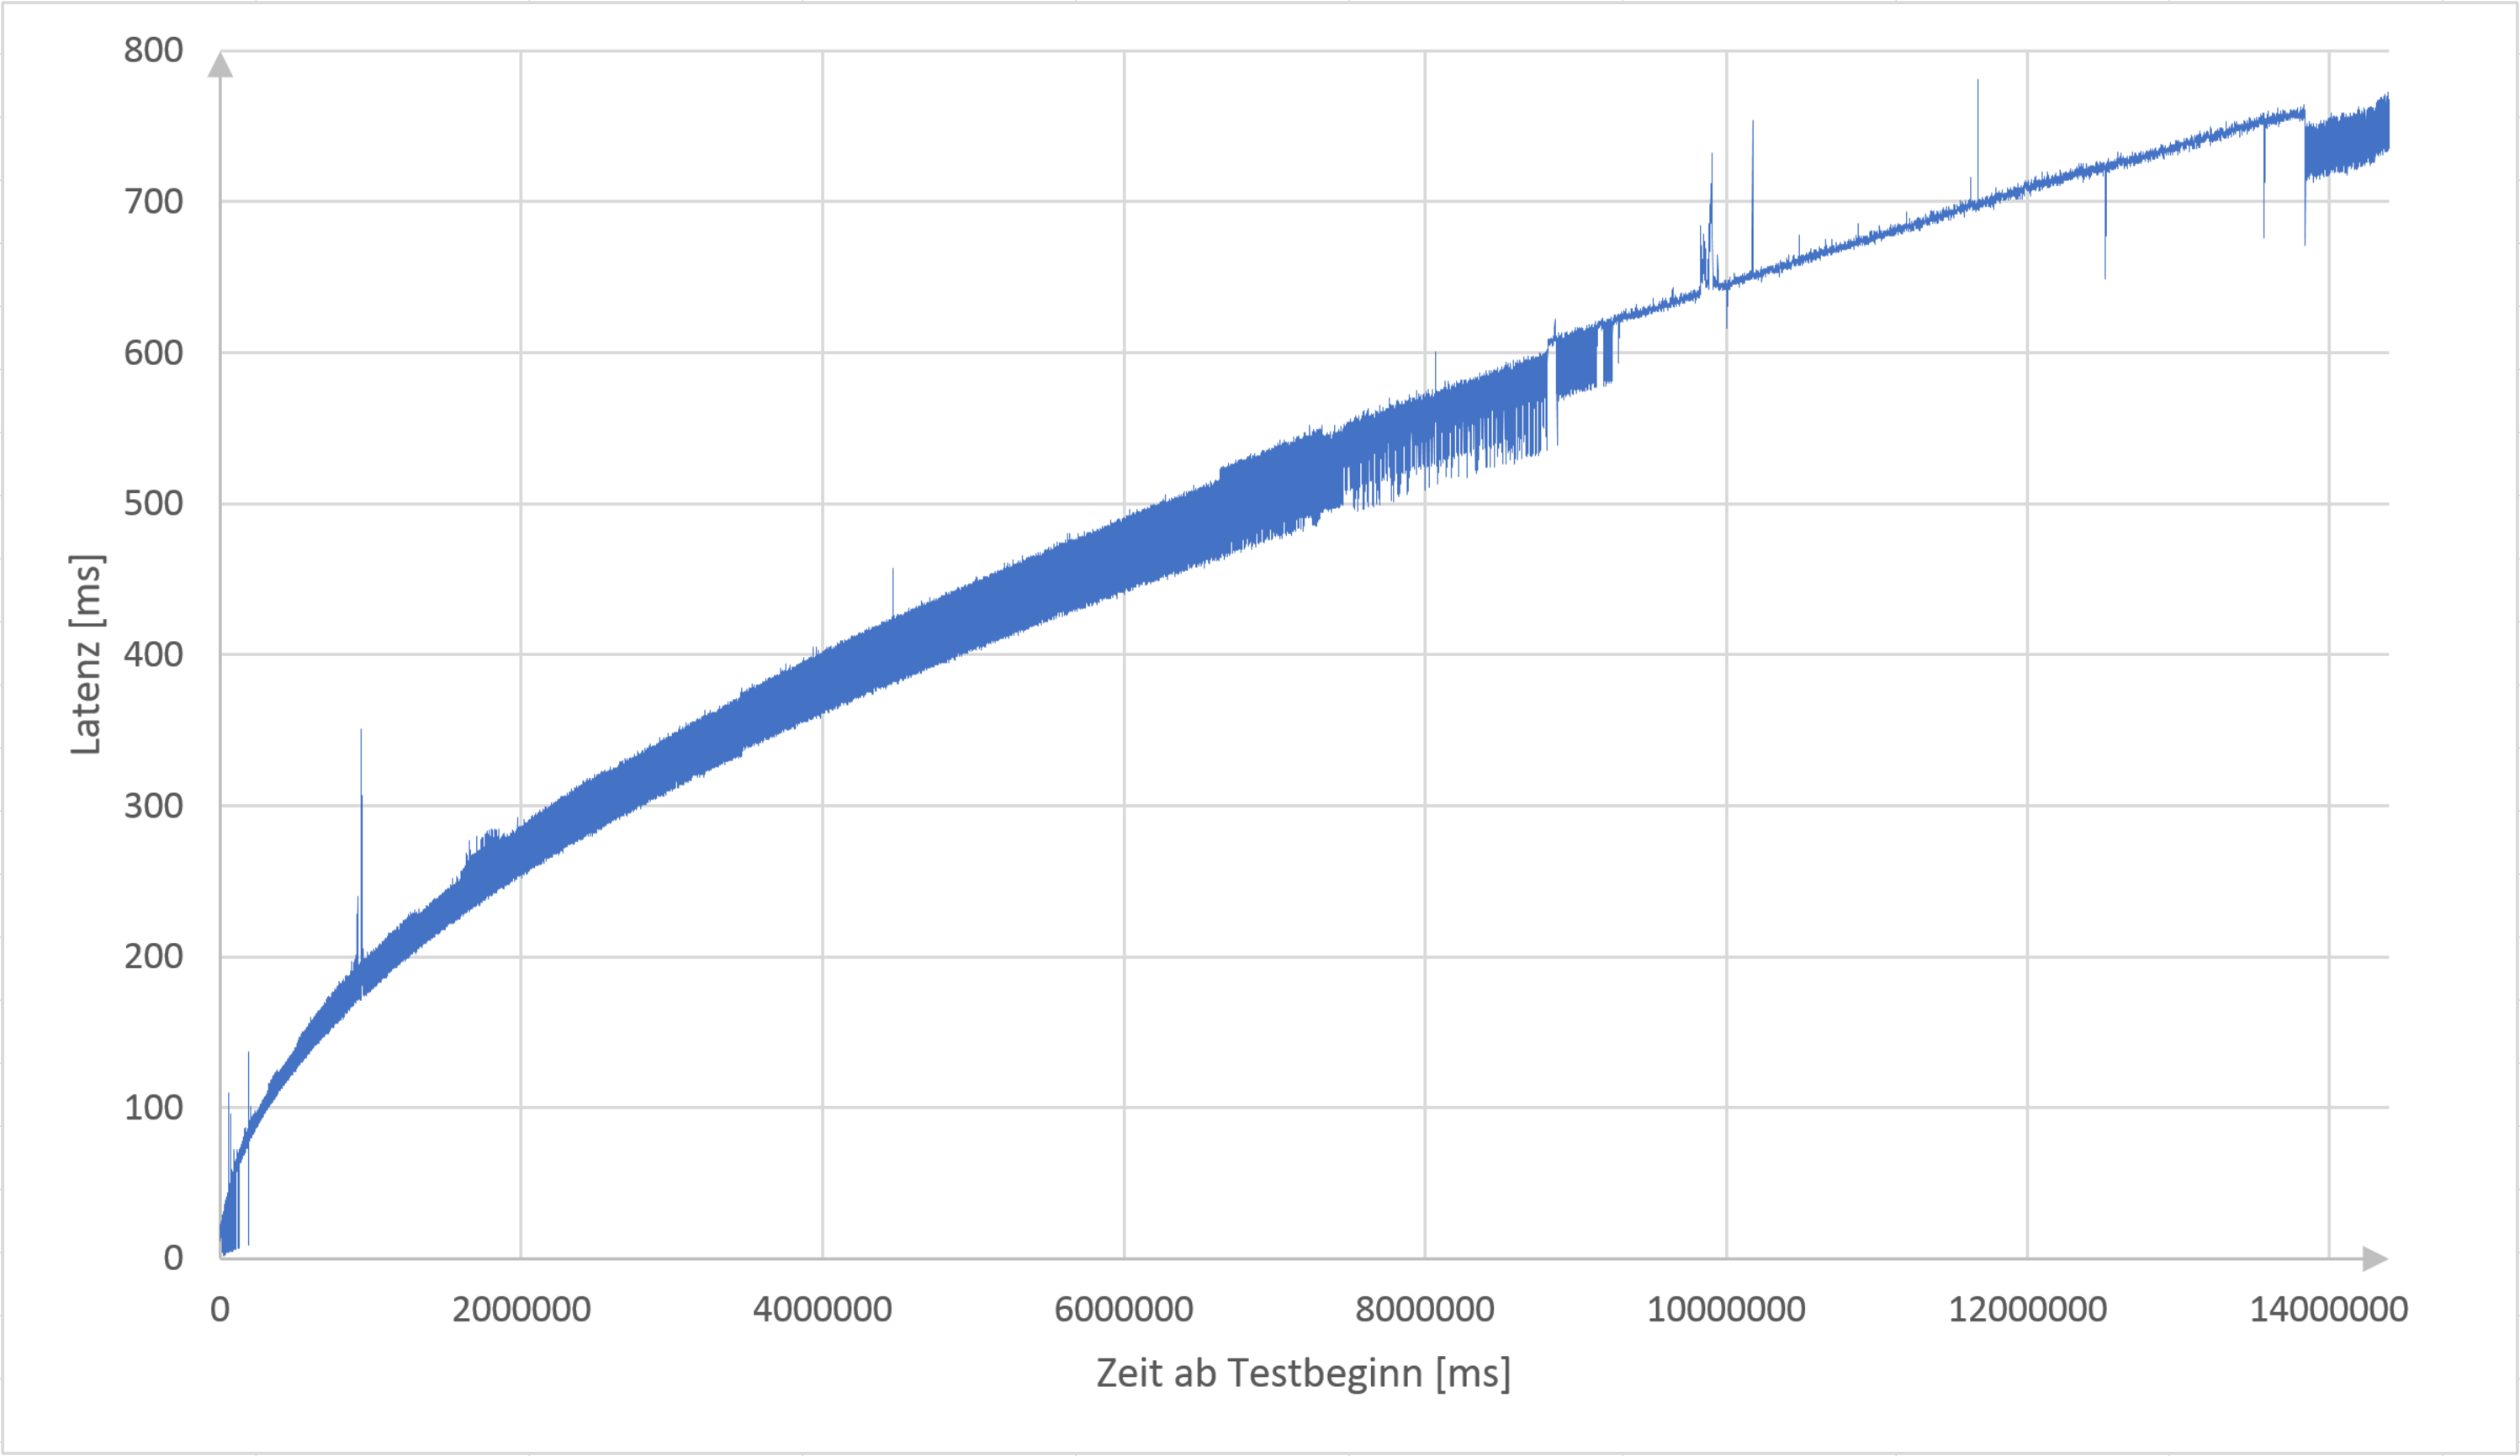
\includegraphics[width=\textwidth]{content/hauptteil/umsetzungPoC/pocTest/res/LatenzNormal4h.pdf}
  \caption{Latenzzeiten im vier Stunden Dauertest}
  \label{fig:testing:latency4hNorm}
\end{figure}
Es fällt auf, dass die Latenz stetig anzusteigen scheint, und sich im gesamten TestVerlauf zwischen \eigenNameNorm{0ms} und \eigenNameNorm{800ms} befindet.
Dieses Verhalten ist nicht erwünscht und wird desshalb genauer untersucht.
Dazu werden die Pakete zwischen den zwei Geräten mit dem Netzwerkanalyseprogramm Wireshark \citep{wireshark:program} mitgeschnitten.
In \refFig{fig:testing:latency4hNorm:wireshark} ist ein Auszug des Mitschnitts dargestellt.
\begin{figure}[ht]
  \centering
  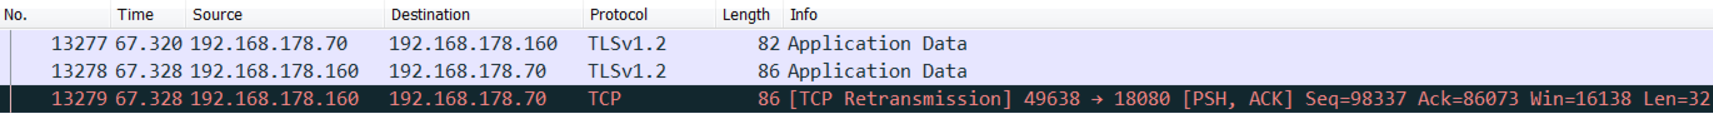
\includegraphics[width=\textwidth]{content/hauptteil/umsetzungPoC/pocTest/res/LatenzNormal4hWireshark.pdf}
  \caption{Auszug aus dem Paketmitschnitt während des vierstündigen Dauertests aus dem Programm \mbox{Wireshark} \citep{wireshark:program}}
  \label{fig:testing:latency4hNorm:wireshark}
\end{figure}
In dem Auszug sieht man den Zeitstempel des Computers mit Windows 7, auf dem Wireshark mitschneidet, die Quelladresse (Source), die Zieladresse (Destination), das Protokoll (Protocol), die Länge (Length), sowie wenige Infos über den Inhalt des Pakets.
Der In \refFig{fig:testing:latency4hNorm:wireshark} dargestellte Auszug wiederholt sich den ganzen Test lang.
Das Backend (IP Adresse: 192.168.178.70) sendet an das Frontend (IP Adresse: 192.168.178.160) eine Websocket Nachricht. Diese ist klein genug, so dass sie in ein Paket passt (Zeile eins).
Die Nachricht kommt im Frontend an. Das ist daran zu erkennen, dass das Frontend darauf (nach ca acht Millisekunde) auf die Nachricht entsprechend des Testskripts antwortet (Zeile zwei).
Daraufhin wird die Nachricht aus Zeile zwei erneut gesendet.
Um diesen Sachverhalt zu erklären, benötigt man es tieferes Verständnis für das \ac{tcp} Protokoll. Genauer wie der Paketaustausch funktioniert und wie Paketverlust verhindert wird.
\begin{figure}[ht]
  \centering
  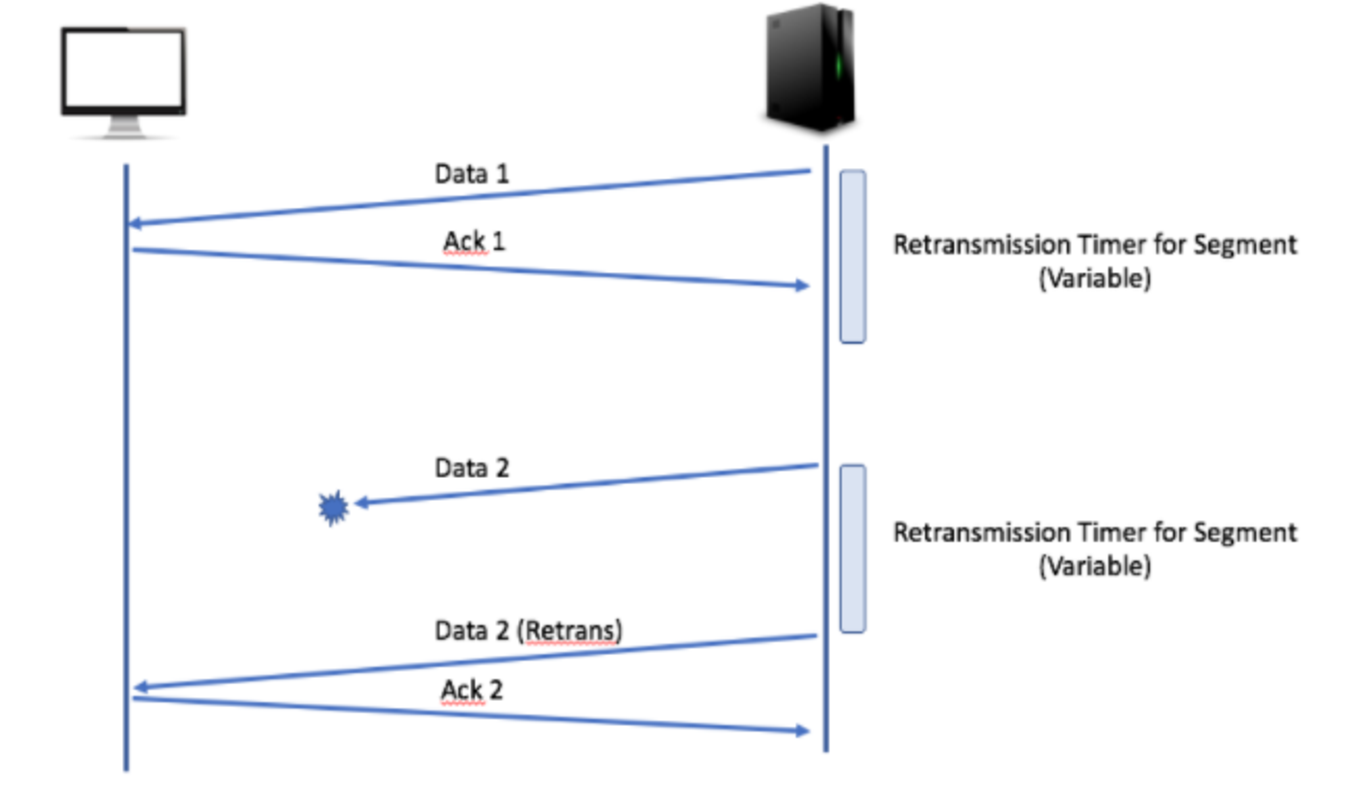
\includegraphics[width=\textwidth]{content/hauptteil/umsetzungPoC/pocTest/res/tcpPackageLostGraph.pdf}
  \caption{Verhalten von \ac{tcp} bei Packetverlust \citep{tcp:articel}}
  \label{fig:testing:tcp:retrans}
\end{figure}
In \refFig{fig:testing:tcp:retrans} ist dargestellt wie der Datenaustausch bei tcp funktioniert.
Immer wenn ein Packet empfangen wird, wird der Empfang des Packets vom Empfänger, durch das Senden eines \acp{ack} an den Sender, bestätigt.
Wenn der Empfang innerhalb einer definierten Zeit (Retransmission Timer in \refFig{fig:testing:tcp:retrans}) nicht bestätigt wird, 
dann wird das Packet wiederholt gesendet.
Diese Zeit in der der Sender auf das \ac{ack} wartet ist nicht konstant und wird entsprechend der Häufigkeit des Auftreten eines ausbleibenden \ac{ack} angepasst.
Bleibt ein \ac{ack} aus, so wird die Zeit sollange erhöht, bis sie so hoch ist, dass sie der doppelten Laufzeit eines Packets auf dem Netzwerk entspricht.
Es ist desshalb die doppelte Zeit, da das gesendete Packet die Zeit des Wegs zum Empfänger braucht und sich dazu die Laufzeit des \ac{ack} zurück zum Sender addiert. Diese Zeit nennt man \ac{rtt}.
Das gilt allerdings nur bei symetrischen Routen zwischen Empfänger und Sender.
Es wird vermutet, dass dieser Regelalgorithmus (congestion control) dafür verantwortlich ist, dass die Latenz stetig ansteigt.
\begin{figure}[ht]
  \centering
  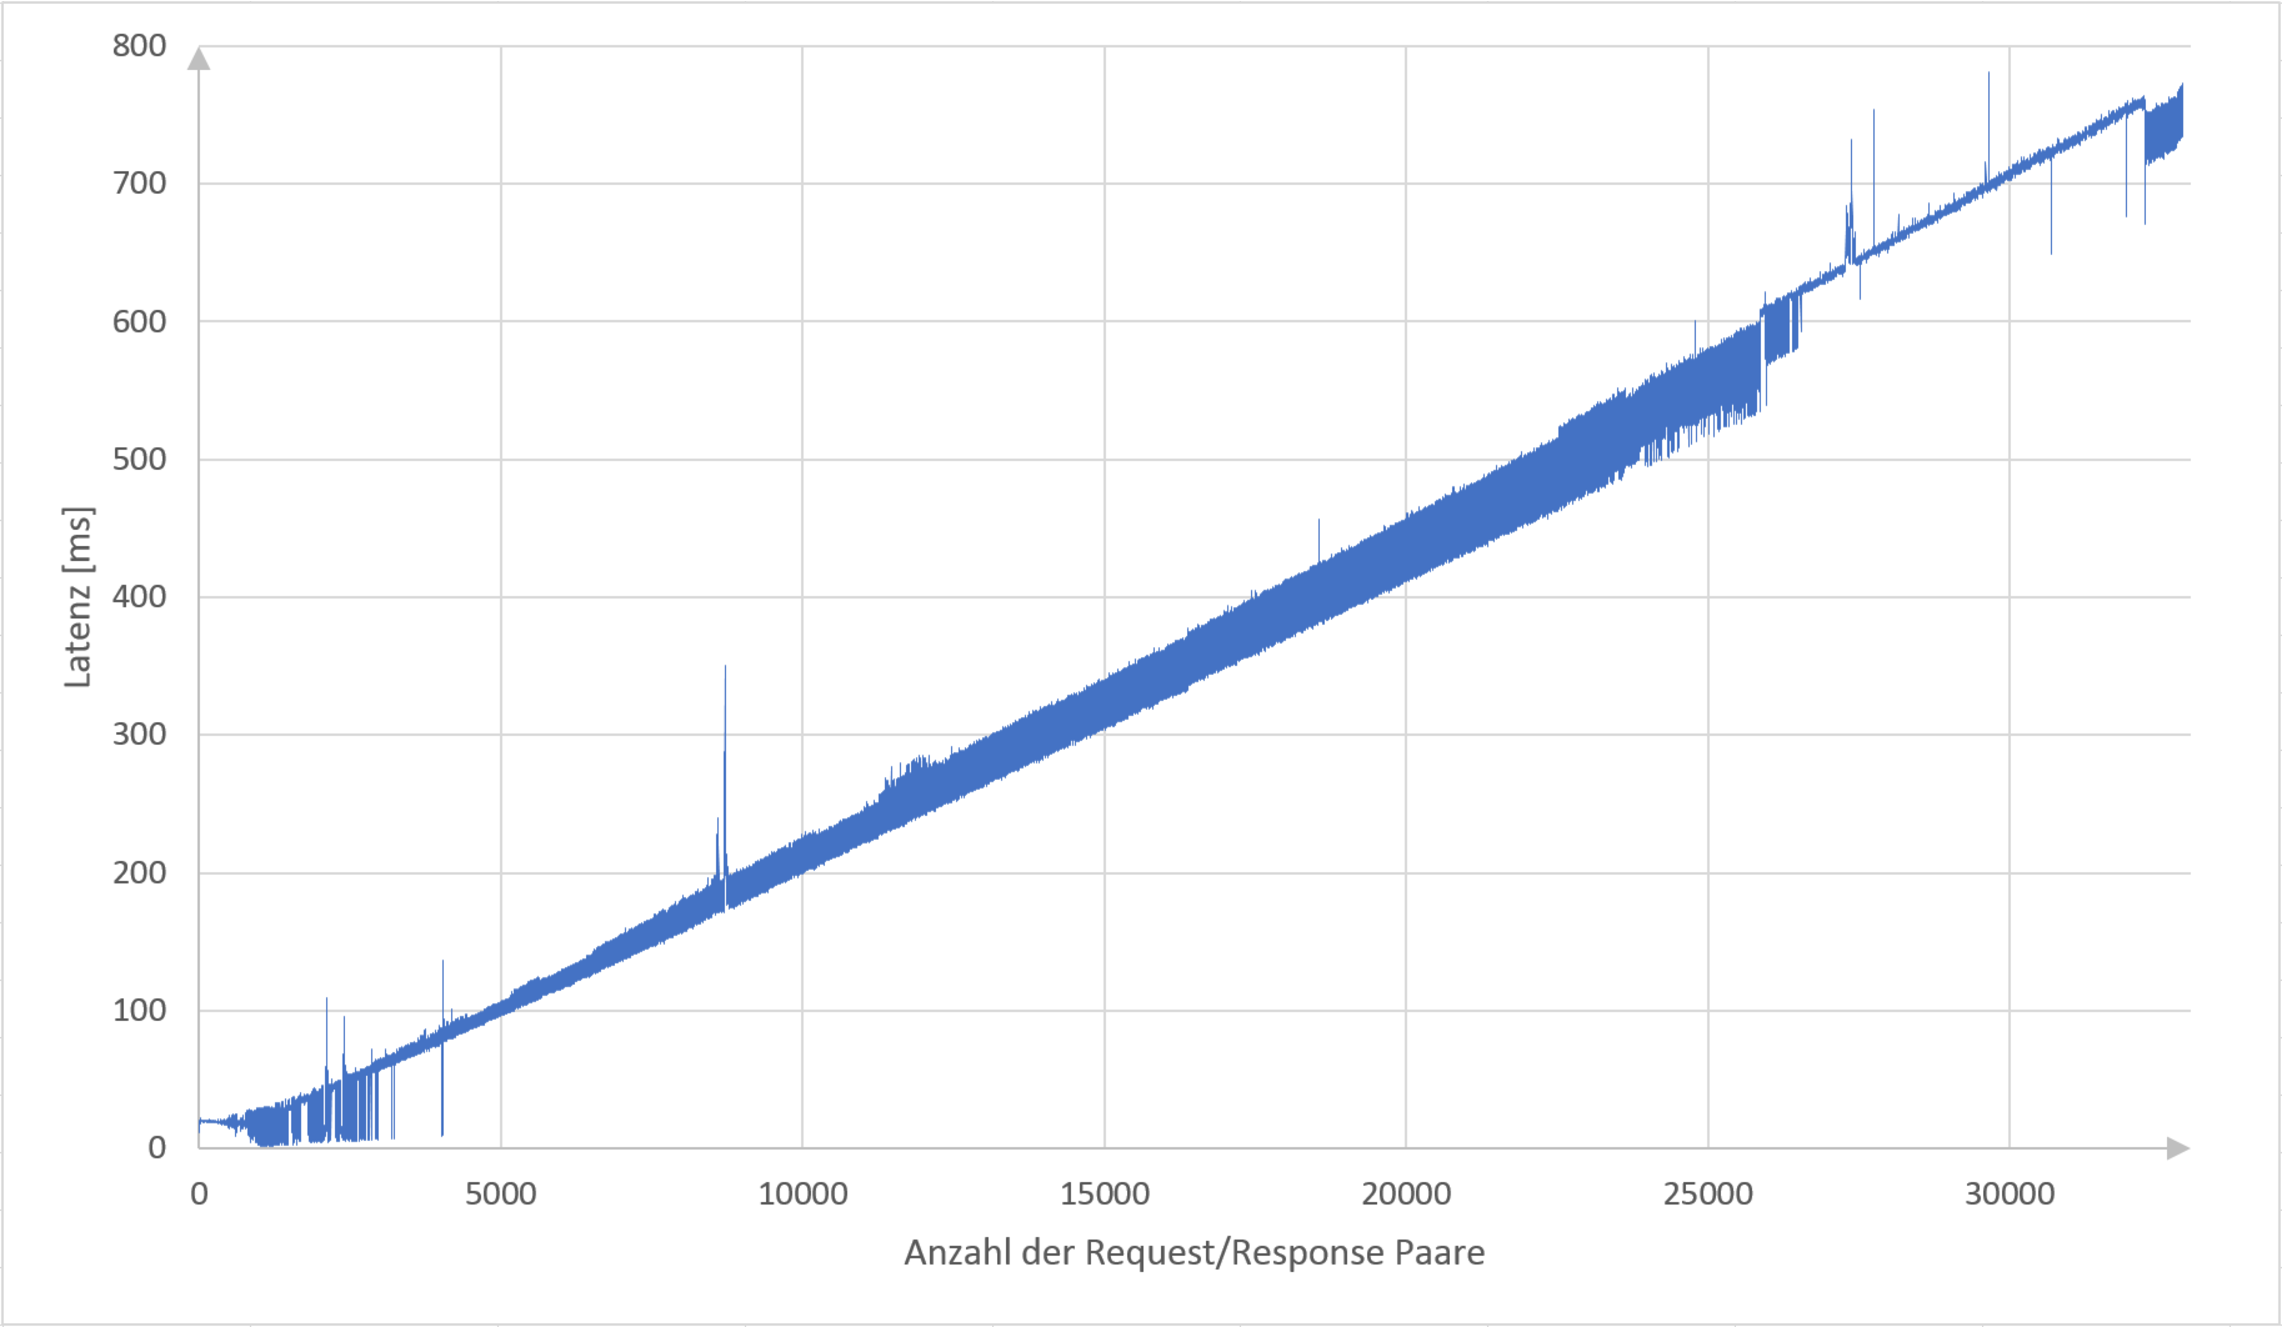
\includegraphics[width=\textwidth]{content/hauptteil/umsetzungPoC/pocTest/res/LatenzNormal4hReqRes.pdf}
  \caption{Latenzzeiten im vier Stunden Dauertest über die Anzahl der vom Backend zum Frontend gesendeten Packeten}
  \label{fig:testing:latency4hNorm:cnt}
\end{figure}
In \refFig{fig:testing:latency4hNorm:cnt} sind nochmal die selben Rohdaten die \refFig{fig:testing:latency4hNorm} zugrunde liegen dargestellt, 
allerdings nun nicht über die Zeit, 
sondern über die Anzahl an vom Frontend an das Backend gesendeten Packeten. 
Hier kann zu Begin, nach der kurzen Konstante innerhalb der ersten 1000 Werte, einen exponentiellen und zum Schluss einen linearen Anstieg erkennen.
Es wird vermutet, dass dies der Regelalgorithmus der Wartezeit auf das \ac{ack} ist und generell Packete vom Fronent zum Backend beim ersten Senden nicht vom Backend bestätigt werden.
Dies würde den wahrscheinlich endlosen Anstieg der Latenz begründen.
Unter der Annahme, dass diese These korrekt ist vermutet der Autor das Problem in der Implementierung einer Websocket Session in der sich senden und empfangen den selben Thread teilen.
Leider kann dieser Sachverhalt aufgrund Zeitmangels nicht weitergehend untersucht werden.
\\Die Echtzeitfähigkeit der Implementierung des aktuellen \ac{poc} ist damit wiederlegt, da die Schnittstelle zwischen Backend und Frontend aufgrund der nicht endlichen Reaktionszeit nicht echtzeitfähig ist.
